\documentclass[12pt, man]{apa6}
\usepackage{graphicx}
\title{Binge Drinking on College Campuses}
\shorttitle{Binge Drinking in College}
\author{John Moon}
\affiliation{San Jose State University}
\date{09-16-2015}

\begin{document}
\maketitle

Across the globe, young adults are leaving home for the first time to attend the university they were accepted to. With this transition comes more freedom than they've ever had in their lives, and an abundance of friends over the legal drinking age. For many students, this creates a "perfect storm" for a frequently occuring activity: binge drinking. While drinking heavily in college is socially acceptablefor the most part, there are many negative aspects involved with it. This paper will examine the cultural feelings, attitudes, and behaviors of students who drink in college. It will take a narrower view to more specifically look at the culture of university students in the United States.

\section{Drinking Culture}
In the United States, the drinking age is 21-years-old. When students are in high school, they become curious about the use of alcohol and want to start using it recreationally. In 2013, a survey of high school students found that 35\% of students had drank some amount of alcohol in the past 30 days, and 21\% of them had binge drank (CDC, 2014). This indicates that a large propotion of high school students in the U.S. are intrigued by the use of alcohol. The taboo nature of drinking is attractive to adolescents as it projects an air of rebellion - a common trait in people this age.

Outside of the U.S., it's uncommon to see a drinking age higher than 18-years-old. One study found that in Europe, teens in high school have drinking events more often than than those in the U.S., however these events have ``fewer occasions of dangerous intoxication''. In Europe, 10\% of those drinking occasions result in intoxication while 50\% of drinking events in the U.S. result in intoxication high school students get to college, they're able to make their own decisions. Without their parents around, these students have far fewer inhibitions when it comes to drinking. Nationally, we see that, ``between 25 and 30 percent of college students drink alcohol at a level that is regarded as problematic in the general population'' (Villanova). Additionally, approximately 70\% of college students report using alcohol in a non-problematic nature.

It's clear that there's a certain attraction that college students have to binge drinking. The environment is perfect for the activity, the social norms are in place, and the developmental state of many students lends itself to being a little bit reckless. But just how much does this cultural perception of binge drinking effect the actual feelings that students have towards it?

\section{Students' Feelings on Binge Drinking}
Peer pressure affects all of us throughout our lives. Sometimes, especially in college, students will participate in an activity simply because their peers are participating. Binge drinking takes place every weekend on campuses across the country. Every student has their reasons for participating, but the most common ones can be pinpointed. In a study conducted by University of Minnesota (2013), they found that the following percentages of students on college campuses believe drinking has these effects:
\begin{itemize}
	\item Breaks the ice: 74.4\%
	\item Enhances social activity: 74.4\%
	\item Gives people something to do: 71.7\%
	\item Gives people something to talk about: 66.6\%
	\item Allows people to have more fun: 63.1\%
	\item Facilitates male bonding: 60.1\%
	\item Facilitates a connection with peers 61.7\%
	\item Facilitates sexual opportunities: 53.0\%
	\item Facilitates female bonding: 28.8\%
	\item Makes women sexier: 28.8\%
	\item Makes food taste better: 22.7\%
	\item Makes me sexier: 20.4\%
	\item Makes men sexier: 19.9\%
\end{itemize}

It seems that students have the general feeling that drinking acts as a social lubricant of sorts. It releases them from feeling the awkward, shy feelings that we've all felt during developmental stages. These are perfectly valid reasons for imbibing, but what leads students to drinking more heavily - to the point where it's considered unhealthy?

\section{Drinking Behaviors}
The decision to drink beyond what's considered a reasonable amount isn't really a decision at all. As one's blood alcohol level rises above 0.06\%, judgement becomes inpaired. This means that when someone is already drunk, the decision to drink more isn't processed by the same standard of reasonability that it would be when the person is sober (Rayner, 2001).

Now, it's interesting to see what exactly sparks a student's drinking any given night. Where do they go to drink? Often, students below the drinking age are not able to go to public bars or purchase their own alcohol, so many of them will go to off-campus house parties to get their alcohol. In an excellent study conducted by Harvard (2001), we see this detailed in the following table:\\
\vspace{5 mm}
\centerline{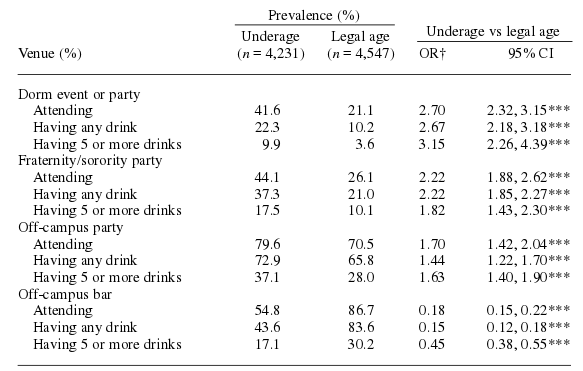
\includegraphics[scale=0.45]{/home/john/.HS1/Locations2.png}}

As one might expect, underage students are found out at off-campus bars less often than students who are of age. It's interesting to note that off-campus parties are a popular destination for both underage and of age students. For the most part, we can also see that once students turn 21, they seem to drink less and less often. This could be due to the ready availability of alcohol (making drinking a less rebellious activity), or perhaps simple maturity.

\section{Attitudes Toward Drinking}
According to a study conducted by the University of New Hampshire, the biggest factor that influences a given student's attitude toward alcohol is how their friends behave (Gaines, 2014). For example, if an underaged student's best friend offers them a drink and claims it isn't a big deal, that student is more likely to have a positive or at least ambivilant perception of underage drinking. Another large factor is how parents have influenced the student. Parents who are more restrictive about alcohol tend to produce children who rebel more once they are able. Conversely, if parents are open and understanding about alcohol use, their children are less likely to abuse alcohol in college.

\section{Discussion}
While binge drinking can be extremely dangerous and lethal in some cases, students across the country still binge drink every weekend. The college culture heavily promotes drinking and there are many factors that influece students' perception on the issue. Especially in the United States, drinking is something college students are just \textit{supposed to do}. However, the majority of students are typically able ot drink a reasonable amount of alcohol, and that's very encouraging.

\newpage
\centerline{References}
\noindent{Brody, Jane E. (2008). Curbing Binge Drinking Takes Group Effort. \textit{The New York Times}.}

\noindent{CDC (2014). Fact Sheets - Underage Drinking. \textit{Center for Disease Control and Prevention}.}

\noindent{Department of Family Social Science (2013). Why Students Drink. \textit{University of}}\\
\textit{Minnesota}.

\noindent{Gaines, Laura (2014). Student Attitudes Towards Drinking Behaviors. \textit{University of New}}\\
\textit{Hampshire}.

\noindent{Rayner, Leah (2001). Alcohol Consumption in College: Losing a Sense of Self. \textit{Bryn Mawr}}\\
\textit{College}.

\noindent{Villanova University. Alcohol Use in College. \textit{Villanova University Student Life}.}

\noindent{Wechsler, Henry, Lee, Jae Eun, Nelson, Toben F., \& Kuo, Meichun (2001). Underage}\\
College Students' Drinking Behavior, Access to Alcohol, and the Influence of\\
Deterrence Policies. \textit{Journal of American College Health}, 50(5).

\end{document}
